
%(BEGIN_QUESTION)
% Copyright 2014, Tony R. Kuphaldt, released under the Creative Commons Attribution License (v 1.0)
% This means you may do almost anything with this work of mine, so long as you give me proper credit

Suppose this generator suffers a ground fault in its left-hand winding.  Assuming a balanced line current of 150 amps through each phase of the 52-P circuit breaker, a ground fault current magnitude of 10 amps, and CT ratios of 200:5, calculate the amount of current going through each coil (RC and OC) of the 87-3 relay:

$$\includegraphics[width=15.5cm]{i00853x01.eps}$$

\underbar{file i00853}
%(END_QUESTION)





%(BEGIN_ANSWER)

Sketching the 150 amp phase current through the breaker and the 10 amp ground fault current reveals 160 amps through the lower phase wire at the bottom of the generator:

$$\includegraphics[width=15.5cm]{i00853x02.eps}$$

200:5 ratios at each CT means the 150 amps through the upper CT will translate into 3.75 amps through the upper restraint coil (RC) of the 87-3 relay.  160 amps through the lower CT translates into 4.00 amps through the lower restraint coil (RC) of the 87-3 relay.  The difference between these two RC currents (0.25 amps) must flow through the 87-3 relay's operate coil (OC).

%(END_ANSWER)





%(BEGIN_NOTES)


%INDEX% Electric power systems: protective relays (differential)
%INDEX% Electronics review: current transformer (CT)
%INDEX% Protective relay: differential current (87)

%(END_NOTES)

